\subsection{Introduction to URBS}
An Uniform Rational Basis Spline (URBS) is a way of expressing a complex path with a small data set. An URBS curve consists of two main components; control points and basis splines.
Control points are a set of locations in space which are individually weighted and summed in order to give the path that the curve travels. They are represented mathematically by the symbol $\textbf{N}^n_i$, where $n$ represents the dimension of the control point and $i$ is an indexing identifier.
Basis splines calculate the weightings that each control point will be given at each point along the curve. As the curve progresses, each spline rises and falls in magnitude. At any point on the curve, the total sum of the magnitudes of all the splines is one.
The higher a control point is weighted, the closer the curve will approach to its location. The first and the last control points are the only points ever to have a weighting of one - meaning that their positions are actually on the curve. Every other control point is weighted in an identical fashion with its influence beginning at zero, rising quadratically to a maximum of 0.75, before again fading to zero. Weightings at specific points along the curve are represented mathematically by the symbol $\textbf{W}_i^d$ where $d$ represents the order of the polynomial that defines the weighting curve and $i$ is an indexing identifier.

In order to display the power of an URBS curve, a demonstrative example is shown in Fig.~\ref{fig:urbsDemo}. The curve can be seen to touch the first and the last control points, but does not ever reach the middle two. The point halfway along the curve is a special point known as a 
knot. A longer curve might have many more of these knot points. Each knot point is a place where a control point's weighting becomes zero and its position will no longer have an effect on the path that the curve takes. As this knot exits, so another enters, with another control point beginning from zero weighting and growing in weighting as the curve continues. At these point the two control points with non-zero weighting are weighted evenly and as such the curve lies directly between them.

A point along the horizontal axis of the spline graph seen in Figure ~\ref{fig:urbsDemo} corresponds to a point on the curve. Since in our application we desire to travel along a path characterised by a URBS curve, we use a parametrisation for each of these points denoted by $s$. Henceforth we often desire to measure the progress made along the path over time. This makes it natural to have $s$ become a function of time $s(t)$. In all instances, $s$ begins a curve at zero and completes a curve when $s$ equates to one. Thus;
\begin{align*}
s(t) &\in [0,1]\\
s(t_0) &= 0\\
s(t_f) &= 1\\
\end{align*}
Where $t_0$ denotes the starting time for the travelling of a path and $t_f$ denotes the finishing time.


\begin{figure}  
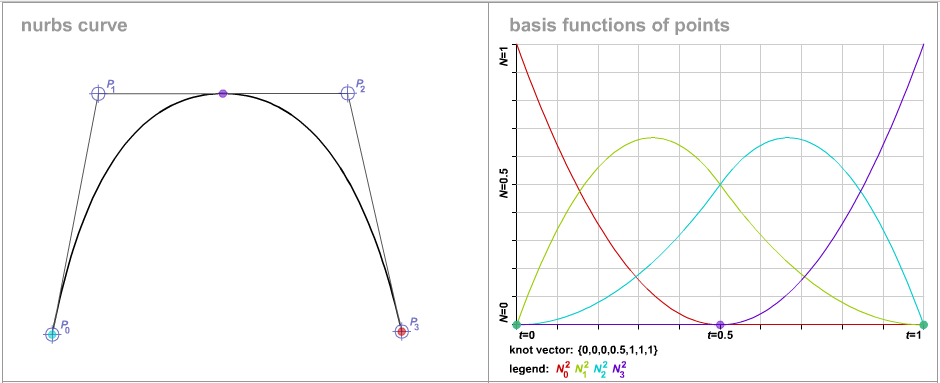
\includegraphics[width=\textwidth]{figures/systemDesign/urbsDemo.png}
\caption[3rd order (Quadratic) URBS curve and corresponding basis splines]{The splines in the right section represent the weighting and mixing of each of the four control points in order to form the curved line seen alongside those points in the left section.\cite{website:nurbsDemo}  
\label{fig:urbsDemo}}
\end{figure}
